\documentclass{article}

\usepackage{amssymb}
\usepackage[polish]{babel}
\usepackage[utf8]{inputenc}
\usepackage{polski}


\usepackage{amsmath}
\DeclareMathOperator{\sgn}{sgn}

\usepackage{pgfplots}
\pgfplotsset{compat=1.17}

\graphicspath{ {./images/} }
\usepackage{lipsum}
\usepackage{caption}
\usepackage{float}

\title{Klasyfikacja COVID-19 na zdjęciach rentgenowskich}
\author{Vladyslav Diachuk s18901}

\bibliographystyle{plain}

\makeindex
\begin{document}
\maketitle

%===================================================================================
\section{Wstęp}

%-----------------------------------------------------------------------------------
\subsection{Abstrakt}


%-----------------------------------------------------------------------------------
\subsection{Słowa kluczowe}


%-----------------------------------------------------------------------------------
\subsection{Teza główna}

%-----------------------------------------------------------------------------------
\subsection{Motywacja}


%===================================================================================
\section{Choroby płuc, rozpoznawanie, skutki}

%===================================================================================
\section{Uczenie maszynowe}
Uczeniem maszynowym nazywa się dziedzina nauki (i sztukę) programowania komputerów w sposób umożliwiający im uczenie się z danych \cite{geron} 
Ta praca jest zrobiona z użyciem uczenia maszynowego a zwłaszcza sieci neuronowych.


%===================================================================================
\section{Neuron}
Zanim opiszę sieci neuronowe, chcę przedstawić co to jest neuron (komórka).

\subsection{Neuron biologiczny}
Jak wiadomo mózg ludzki i większości innych organizmów składa się z malutkich komórek nerwowych, nazywanych neuron, zdolnych do przetwarzania i przewodzenia informacji w postaci sygnału elektrycznego. Neurony są podstawowym elementem układu nerwowego zwierząt. Najwięcej neuronów znajduje się w ośrodkowym układzie nerwowym, w skład którego wchodzi mózgowie oraz rdzeń kręgowy. \cite{neuroscience}
Głównymi elementami neuronu są ciało komórki zawierające jądro i większość organelli komórkowych, wiele rozgałęziających się wypustek zwanych dendrytami oraz jedna bardzo długa wypustka -- akson. \cite{geron}

\begin{figure}
	\centering
	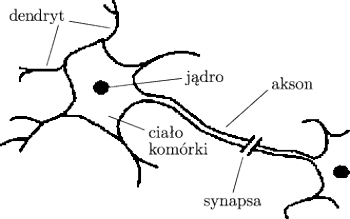
\includegraphics[width=\textwidth,height=6cm,keepaspectratio=true]{neuron_bio}
	\caption{
		Obraz komórki biologicznej \cite{neuron_bio}
	}
\end{figure}

Neurony biologiczne generują krótkie impulsy elektryczne zwane sygnałami, które są przenoszone wzdłuż aksonów i powodują uwalnianie w synapsach sygnałów chemicznych zwanych neuroprzekaźnikami. Kiedy komórka nerwowa otrzymuje dostateczną liczbę neuroprzekaźników od innych neuronów w ciągu kilku milisekund, to sama zaczyna wysyłać własne sygnały elektryczne (w rzeczywistości jest to uzależnione od neuroprzekaźników, gdyż niektóre z nich hamują aktywność komórki nerwowej). \cite{geron}
Zatem mechanizm działania poszczególnych neuronów jest dość prosty, tworzą one jednak rozległą sieć składającą się z miliardów komórek nerwowych, gdzie zazwyczaj jeden neuron łączy się z tysiącami innych. Dzięki tak olbrzymiej sieci zawierającej proste komórki nerwowe mogą być wykonywane skomplikowane obliczenia.

\subsection{Sztuczny neuron}
W 1943 przez Warren S. McCulloch i Walter Pitts było zaproponowano bardzo prostą reprezentację neuronu sztucznego. On ma co najmniej jedno binarne wejście i dokładnie jedno binarne wyjście. Wyjście zostanie aktywne tylko wtedy kiedy będzie aktywna określona liczba wejść. \cite{mcculloch1943logical} Tak prosty model daje nam bardzo duże możliwości. Twórcy udowodnili że za pomocą takich neuronów jesteśmy w stanie zaprotestować sieć która rozwiąże dowolne zadanie logiczne.

\clearpage
	
\begin{figure}
	\centering
	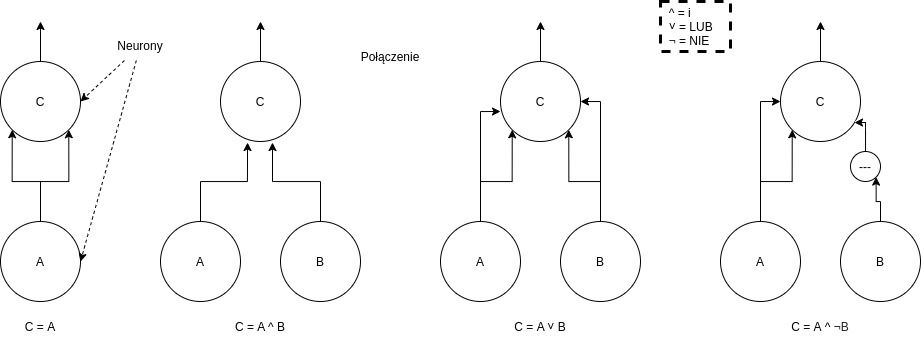
\includegraphics[width=\textwidth,keepaspectratio=true]{SSN_simple_neurons}
	\caption{
		Przykład sztucznych sieci neuronowych przeprowadzających proste operacje logiczne. Neuron aktywuje się przy co najmniej dwóch aktywnych wejściach \cite{geron}
	}
\end{figure}

Frank Rossenblatt trochę zmodyfikował ten neuron.\newline
Kluczowe zmiany:
\begin{itemize}
	\item Wartościami wejść/wyjść są liczby
	\item Każde połączenie ma przyporządkowaną wagę.
	\item Używanie funkcji skokowej na końcu
	\item Dodatkowe obciążeniowe wejście(zawsze wysyła wartość 1) z własną wagą, tak zwany bias
\end{itemize}
Jednostka wylicza ważoną sumę sygnałów wejściowych, a następnie zostaję użyta funkcja aktywacji. Najczęściej zostaje użyta funkcja skokowa Heaviside`a (Rysunek \ref{Heaviside}) lub signum (Rysunek \ref{Signum}) .Przy użyciu skokowej funkcji aktywacji taki neuron można nazywać progową jednostką logiczną lub liniową jednostką progową (ang. \textit{Linear Treshod Unit} -- LTU). Dziawanie tej jednoki można matematycznie opisać w następujący sposób.\newline\newline
$ y = \mathcal{H}(W^{T}X + b) $\newline \newline
Gdzie: \newline
X -- wektor wejść. \newline
W -- wektor wag. \newline
b -- bias. \newline
y -- wyjście neuronu. \newline
$ \mathcal{H}(...) $ -- funkcja skokowa Heaviside`a\newline

\begin{figure}[H]
	\centering
	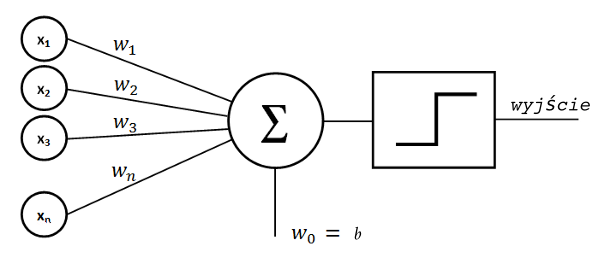
\includegraphics[width=0.8\textwidth,keepaspectratio=true]{neuron_rosenblatta}
	\captionof{figure}{
		Sztuczny neuron Franka Rosenblatta
	}
\end{figure}




%===================================================================================
\section{Funkcji aktywacji użyte w pracy}

%-----------------------------------------------------------------------------------
\subsection{Funkcja skokowa Heaviside’a}
Funkcja skokowa Heaviside’a, skok jednostkowy – funkcja nieciągła, która przyjmuje wartość dla ujemnych argumentów i wartość 1 w pozostałych przypadkach:

\begin{equation}
	\mathcal{H}(x) = 
	\begin{cases}
		0 & \text{dla $x < 0$}\\
		1 & \text{dla $x \geqslant 0$ }\\
	\end{cases}    
\end{equation}

\begin{figure}[H]
	\centering
	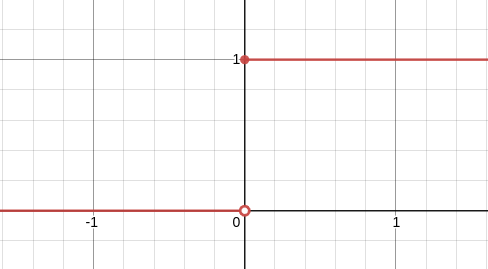
\includegraphics[width=0.6\textwidth,keepaspectratio=true]{Heaviside}
	\caption{
		Funkcja skokowa Heaviside’a
	}
	\label{Heaviside}
\end{figure}


%-----------------------------------------------------------------------------------
\subsection{Signum}
Signum, sgn (łac. signum „znak”) – funkcja zmiennej rzeczywistej, zdefiniowana następująco:
\begin{equation}
	sgn(x) = 
	\begin{cases}
		-1 & \text{dla $x < 0$}\\
		0 & \text{dla $x = 0$}\\
		1 & \text{dla $x > 0$}\\
	\end{cases}    
\end{equation}

\begin{figure}[H]
	\centering
	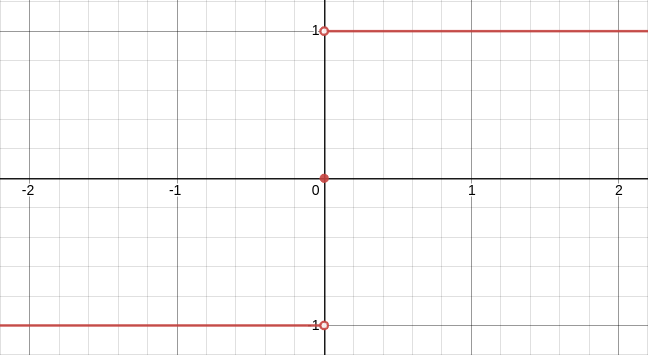
\includegraphics[width=0.6\textwidth,keepaspectratio=true]{Signum}
	\caption{
		Signum
	}
	\label{Signum}
\end{figure}


%-----------------------------------------------------------------------------------
\subsection{Sigmoid}
Funkcja sigmoidalna jest funkcją matematyczną mającą charakterystyczną krzywą w kształcie litery „S” lub krzywą sigmoidalną.
Typowym przykładem funkcji sigmoidalnej jest funkcja logistyczna pokazana na rysunku \ref{Sigmoid} i zdefiniowana wzorem: 

$S(x) = \dfrac{1}{1 + e^{-x}}$

\begin{figure}[H]
	\centering
	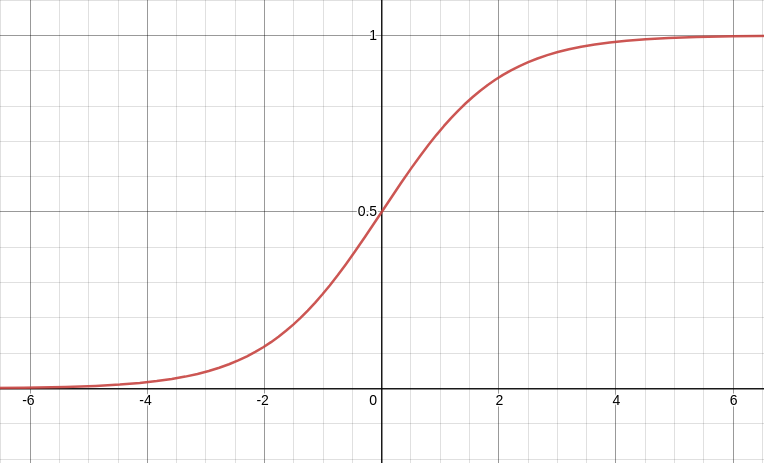
\includegraphics[width=0.6\textwidth,keepaspectratio=true]{Sigmoid}
	\caption{
		Sigmoid
	}
	\label{Sigmoid}
\end{figure}

%-----------------------------------------------------------------------------------
\subsection{ReLU}
Kolejną, popularną funkcją aktywacji jest ReLU (rectifier Linear Unit). Od swojego kształtu w mowie potocznej często nazywana jest funkcją rampy (bo i rzeczywiście - wygląda jak rampa).
\begin{equation}
	ReLU(x) = 
	\begin{cases}
		0 & \text{dla $x < 0$}\\
		x & \text{dla $x \geqslant 0$ }\\
	\end{cases}    
\end{equation}

\begin{figure}[H]
	\centering
	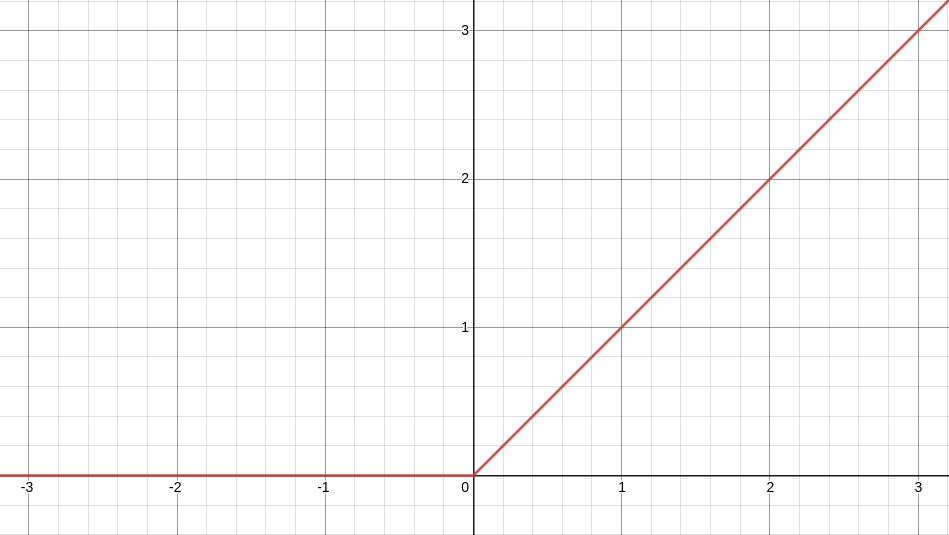
\includegraphics[width=0.6\textwidth,keepaspectratio=true]{ReLu}
	\caption{
		ReLU
	}
\end{figure}

%===================================================================================
\section{Sieci neuronowe w klasyfikacji danych wizualnych}

%-----------------------------------------------------------------------------------
\subsection{Model neuronu jako klasyfikator}

%-----------------------------------------------------------------------------------
\subsection{Konwolucyjne sieci neuronowe}

%-----------------------------------------------------------------------------------
\subsection{Uczenie sztucznych sieci neuronowych}



%===================================================================================
\section{Architektura konwolucyjna w detekcji chorób płuc}



\bibliography{bibliografia}

	
\end{document}